%%%%%%%%%%%%%%%%%%%%%%%%%%%%%%%%%%%%%%%%%%%%%%%%%%%%%%%%%%%%%%%%%%%%%%%%%%%%%%%%%%%%%%%%%%%%%%%%%%%%%%%%%%%%%%%%%%%%%%%%%%%%%%%%%%%%%%%%%%%%%%%%%%%%%%%%%%%%%%%%%%%
% Written By Michael Brodskiy
% Class: Modern Physics
% Professor: Q. Yan
%%%%%%%%%%%%%%%%%%%%%%%%%%%%%%%%%%%%%%%%%%%%%%%%%%%%%%%%%%%%%%%%%%%%%%%%%%%%%%%%%%%%%%%%%%%%%%%%%%%%%%%%%%%%%%%%%%%%%%%%%%%%%%%%%%%%%%%%%%%%%%%%%%%%%%%%%%%%%%%%%%%

\include{Includes.tex}

\title{Homework 7}
\date{April 9, 2023}
\author{Michael Brodskiy\\ \small Professor: Q. Yan}

\begin{document}

\maketitle

\newpage

\begin{enumerate}

    \section{Symmetric Quantum Well}

  \item 

    \begin{enumerate}

      \item If $|\psi(x)|^2$ is symmetric (as specified), then $\psi(x)$ is symmetric about the origin as well. We know that $\psi(-x)=\psi(x)$ or $\psi(-x)=-\psi(x)$. If neither of these cases is true, then $|\psi(x)|^2$ can not be symmetric. For example, if $\psi(-x)\neq\psi(x)$, then:

        $$|\psi(x)|\neq|\psi(-x)|$$

        This means:

        $$|\psi(x)|^2\neq|\psi(-x)|^2$$

        which contradicts the symmetry of $|\psi(x)|^2$

        Additionally, if $\psi(-x)\neq-\psi(x)$, the process becomes similar, as $-\psi(x)$ becomes positive due to the absolute value sign.

        Thus, it is necessary that $\psi(-x)=\psi(x)$ or $\psi(-x)=-\psi(x)$, so that $|\psi(x)|^2$ maintains its symmetry.

      \item Assuming the solution to the function is $A\cos(kx)+B\sin(kx)$, and knowing that $U(x)$ is zero:

        $$\frac{\partial^2\psi}{\partial x^2}=-Ak^2\cos(kx)-Bk^x\sin(kx)$$
        $$\frac{\partial^2\psi}{\partial x^2}=-k^2\psi(x)$$

        Thus, we get:

        $$\frac{\hbar^2k^2}{2m}\psi(x)=E\psi(x)$$
        $$k=\frac{\sqrt{2mE}}{\hbar}$$

        Given the above functions, we know that $k$ must be:

        $$k=\frac{n\pi}{L},\quad\quad n=1,2,3,\cdots$$

        Using boundary conditions at $\frac{L}{2}$:

        $$\psi\left( \frac{L}{2} \right)=A\cos\left( \frac{n\pi}{2} \right)+B\sin\left( \frac{n\pi}{2} \right)$$

        When $n$ is odd, this means $A=0$, as $\cos$ goes to zero, and, due to boundary conditions, $B=0$ as well; when $n$ is even, this means $B=0$ as $\sin$ goes to zero, and, due to boundary conditions, $A=0$ as well. Now applying normalization:\\

        When $n$ is odd:

        $$\int_{-\frac{L}{2}}^{\frac{L}{2}}|B\sin\left( \frac{2\pi x}{L} \right)|^2\,dx=1\Rightarrow b=\sqrt{\frac{L}{2}}$$

        When $n$ is even:

        $$\int_{-\frac{L}{2}}^{\frac{L}{2}}|A\cos\left( \frac{\pi x}{L} \right)|^2\,dx=1\Rightarrow A=\sqrt{\frac{L}{2}}$$

        Thus, the equation becomes:

        $$\left\{\begin{array}{l r} \sqrt{\frac{2}{L}}\cos\left( \frac{n\pi x}{L} \right), & \text{for } n \text{ odd}\\ \sqrt{\frac{2}{L}}\sin\left( \frac{n\pi x}{L} \right), & \text{for } n \text{ even}\\ \end{array}$$

      \item Given the wave functions from (b) and applying them to the wave function:

        $$\left\{\begin{array}{l} \sqrt{\frac{2}{L}}\cos\left( \frac{n\pi x}{L} \right)\rightarrow-\frac{n\pi}{L}\sqrt{\frac{2}{L}}\sin\left( \frac{n\pi x}{L} \right)\rightarrow-\frac{n^2\pi^2}{L^2}\sqrt{\frac{2}{L}}\cos\left( \frac{n\pi x}{L} \right)\\ \sqrt{\frac{2}{L}}\sin\left( \frac{n\pi x}{L} \right)\rightarrow\frac{n\pi}{L}\sqrt{\frac{2}{L}}\cos\left( \frac{n\pi x}{L} \right)\rightarrow-\frac{n^2\pi^2}{L^2}\sqrt{\frac{2}{L}}\sin\left( \frac{n\pi x}{L} \right) \end{array}$$

          Putting this into the wave function, we get:

          $$-\frac{\hbar^2}{2m}\left( -\frac{n^2\pi^2}{L^2}\sqrt{\frac{2}{L}}\sin\left( \frac{n\pi x}{L} \right) \right)=(E-U(x))\sqrt{\frac{2}{L}}\sin\left( \frac{n\pi x}{L} \right)$$

          Canceling out common terms, we get:

          $$E=\frac{\hbar^2n^2\pi^2}{2mL^2}+U(x)$$

          Because $E$ is constant and independent of $x$, and $U(x)$ is zero within the well, the possible energies become:

          $$E=\frac{\hbar^2n^2\pi^2}{2mL^2}$$

    \end{enumerate}

    \section{Speed of Electron in Bohr Model}

  \item 

    \begin{enumerate}

      \item We know that $\alpha=\dfrac{e^2}{4\pi\varepsilon_o\hbar c}$

        Due to the principles of angular momentum, we obtain:

        $$mvr=n\hbar$$

        The radius of the $n$-th state is:

        $$r_n=\dfrac{4\pi\varepsilon_o\hbar^2n^2}{me^2}$$

        Using the two formulas and substituting, we get:

        $$v=\frac{1}{n}\left( \frac{e^2}{4\pi\varepsilon_o\hbar} \right)$$

        Multiplying by $c$, we get:

        $$v=\frac{1}{n}\left( \frac{e^2}{4\pi\varepsilon_o\hbar} \right)\frac{c}{c}$$
        $$v=\frac{c}{n}\left( \frac{e^2}{4\pi\varepsilon_o\hbar c} \right)$$

        And thus, $v$ becomes:

        $$v=\frac{\alpha c}{n}$$

      \item Given a hydrogen-like atom with charge $Ze$, the coulomb force is $Z^2$ times its original value. The radius, however, is decreased by a factor of $Z$, meaning that the velocity becomes:

        $$v_Z=\frac{Z\alpha c}{n}$$

    \end{enumerate}

    \section{Ionized Helium}

  \item Ionized helium energy levels would look as follows:

    \begin{figure}[h!]
      \centering
      \tikzset{every picture/.style={line width=0.75pt}} %set default line width to 0.75pt        

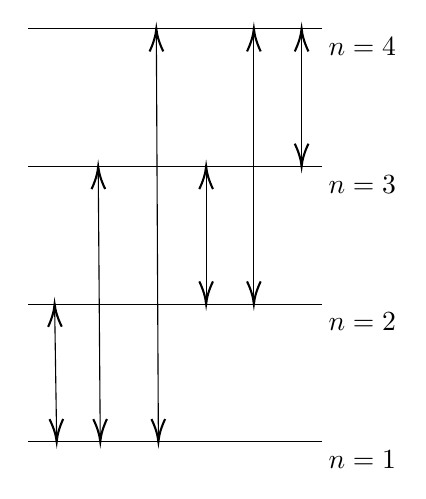
\begin{tikzpicture}[x=0.75pt,y=0.75pt,yscale=-1,xscale=1]
%uncomment if require: \path (0,425); %set diagram left start at 0, and has height of 425

%Straight Lines [id:da10159599772539862] 
\draw    (220.71,109) -- (79.29,109) ;
%Straight Lines [id:da5080837939197953] 
\draw    (220.71,175.33) -- (79.29,175.33) ;
%Straight Lines [id:da9723609878654813] 
\draw    (220.71,241.67) -- (79.29,241.67) ;
%Straight Lines [id:da4964454195724415] 
\draw    (220.71,308) -- (79.29,308) ;
%Straight Lines [id:da15757741863052366] 
\draw    (92.97,306) -- (92.03,243.67) ;
\draw [shift={(92,241.67)}, rotate = 89.14] [color={rgb, 255:red, 0; green, 0; blue, 0 }  ][line width=0.75]    (10.93,-3.29) .. controls (6.95,-1.4) and (3.31,-0.3) .. (0,0) .. controls (3.31,0.3) and (6.95,1.4) .. (10.93,3.29)   ;
\draw [shift={(93,308)}, rotate = 269.14] [color={rgb, 255:red, 0; green, 0; blue, 0 }  ][line width=0.75]    (10.93,-3.29) .. controls (6.95,-1.4) and (3.31,-0.3) .. (0,0) .. controls (3.31,0.3) and (6.95,1.4) .. (10.93,3.29)   ;
%Straight Lines [id:da399415600720878] 
\draw    (113.98,306) -- (113.02,177.33) ;
\draw [shift={(113,175.33)}, rotate = 89.57] [color={rgb, 255:red, 0; green, 0; blue, 0 }  ][line width=0.75]    (10.93,-3.29) .. controls (6.95,-1.4) and (3.31,-0.3) .. (0,0) .. controls (3.31,0.3) and (6.95,1.4) .. (10.93,3.29)   ;
\draw [shift={(114,308)}, rotate = 269.57] [color={rgb, 255:red, 0; green, 0; blue, 0 }  ][line width=0.75]    (10.93,-3.29) .. controls (6.95,-1.4) and (3.31,-0.3) .. (0,0) .. controls (3.31,0.3) and (6.95,1.4) .. (10.93,3.29)   ;
%Straight Lines [id:da39270251068842477] 
\draw    (141.99,306) -- (141.01,111) ;
\draw [shift={(141,109)}, rotate = 89.71] [color={rgb, 255:red, 0; green, 0; blue, 0 }  ][line width=0.75]    (10.93,-3.29) .. controls (6.95,-1.4) and (3.31,-0.3) .. (0,0) .. controls (3.31,0.3) and (6.95,1.4) .. (10.93,3.29)   ;
\draw [shift={(142,308)}, rotate = 269.71] [color={rgb, 255:red, 0; green, 0; blue, 0 }  ][line width=0.75]    (10.93,-3.29) .. controls (6.95,-1.4) and (3.31,-0.3) .. (0,0) .. controls (3.31,0.3) and (6.95,1.4) .. (10.93,3.29)   ;
%Straight Lines [id:da27190914055791304] 
\draw    (165,239.67) -- (165,177.33) ;
\draw [shift={(165,175.33)}, rotate = 90] [color={rgb, 255:red, 0; green, 0; blue, 0 }  ][line width=0.75]    (10.93,-3.29) .. controls (6.95,-1.4) and (3.31,-0.3) .. (0,0) .. controls (3.31,0.3) and (6.95,1.4) .. (10.93,3.29)   ;
\draw [shift={(165,241.67)}, rotate = 270] [color={rgb, 255:red, 0; green, 0; blue, 0 }  ][line width=0.75]    (10.93,-3.29) .. controls (6.95,-1.4) and (3.31,-0.3) .. (0,0) .. controls (3.31,0.3) and (6.95,1.4) .. (10.93,3.29)   ;
%Straight Lines [id:da43254530577246375] 
\draw    (188,239.67) -- (188,111) ;
\draw [shift={(188,109)}, rotate = 90] [color={rgb, 255:red, 0; green, 0; blue, 0 }  ][line width=0.75]    (10.93,-3.29) .. controls (6.95,-1.4) and (3.31,-0.3) .. (0,0) .. controls (3.31,0.3) and (6.95,1.4) .. (10.93,3.29)   ;
\draw [shift={(188,241.67)}, rotate = 270] [color={rgb, 255:red, 0; green, 0; blue, 0 }  ][line width=0.75]    (10.93,-3.29) .. controls (6.95,-1.4) and (3.31,-0.3) .. (0,0) .. controls (3.31,0.3) and (6.95,1.4) .. (10.93,3.29)   ;
%Straight Lines [id:da2755208448822286] 
\draw    (211,173.33) -- (211,111) ;
\draw [shift={(211,109)}, rotate = 90] [color={rgb, 255:red, 0; green, 0; blue, 0 }  ][line width=0.75]    (10.93,-3.29) .. controls (6.95,-1.4) and (3.31,-0.3) .. (0,0) .. controls (3.31,0.3) and (6.95,1.4) .. (10.93,3.29)   ;
\draw [shift={(211,175.33)}, rotate = 270] [color={rgb, 255:red, 0; green, 0; blue, 0 }  ][line width=0.75]    (10.93,-3.29) .. controls (6.95,-1.4) and (3.31,-0.3) .. (0,0) .. controls (3.31,0.3) and (6.95,1.4) .. (10.93,3.29)   ;

% Text Node
\draw (222.71,311) node [anchor=north west][inner sep=0.75pt]   [align=left] {$\displaystyle n=1$};
% Text Node
\draw (222.71,244.67) node [anchor=north west][inner sep=0.75pt]   [align=left] {$\displaystyle n=2$};
% Text Node
\draw (222.71,178.33) node [anchor=north west][inner sep=0.75pt]   [align=left] {$\displaystyle n=3$};
% Text Node
\draw (222.71,112) node [anchor=north west][inner sep=0.75pt]   [align=left] {$\displaystyle n=4$};


\end{tikzpicture}

      \caption{Helium Energy Transition Diagram}
      \label{fig:1}
    \end{figure}

    The major difference between hydrogen and helium is the result of the two protons in the nucleus, which modify the energy levels of each quanta. The energy of each $n$-th orbit is given by:

    $$E_n=-13.6\frac{z^2}{n^2}$$

    Thus, the energies for the different levels, given $z=2$ instead of hydrogen's $z=1$, we obtain:

    $$E_{1,2,3,4}=-54.4,-13.6,-6.04,-3.4[\si{\eV}]$$

    Using the wavelength for emission spectra formula:

    $$\frac{1}{\lambda}=Rz^2\left( \frac{1}{n_1^2}-\frac{1}{n_2^2} \right)$$

    Using a calculator\footnote{GNU Octave}, the following wavelengths are obtained:

    $$\lambda_{1\leftrightarrow2}=30.39[\si{\nano\meter}]$$
    $$\lambda_{1\leftrightarrow3}=25.64[\si{\nano\meter}]$$
    $$\lambda_{1\leftrightarrow4}=24.3[\si{\nano\meter}]$$
    $$\lambda_{2\leftrightarrow3}=164.1[\si{\nano\meter}]$$
    $$\lambda_{2\leftrightarrow4}=121.5[\si{\nano\meter}]$$
    $$\lambda_{3\leftrightarrow4}=468.8[\si{\nano\meter}]$$

    \section{Optical Transition and Momentum Conservation}

  \item The momentum of a photon, given a difference in energy, is:

    $$p=\frac{E_1-E_2}{c}$$

    Conservation of linear momentum means that the atom and photon will have equal but opposite momentums. Using the above momentum in the formula for energy, we get:

    $$K_R=\frac{p^2}{2m}=\frac{(E_1-E_2)^2}{2c^2m}$$

    Therefore, the provided formula is correct in describing the recoil energy:

    $$K_R\cong\frac{(E_1-E_2)^2}{2Mc^2}$$

\end{enumerate}

\end{document}

